\documentclass[11pt,a4paper]{article}
\usepackage[T1]{fontenc}
\usepackage[utf8]{inputenc}
\usepackage{lmodern}
\usepackage{microtype}
\usepackage[a4paper,top=25mm,bottom=26mm,left=27mm,right=27mm]{geometry}
\usepackage{amsmath,amssymb,amsthm,mathtools}
\usepackage{booktabs,tabularx,array}
\usepackage{xcolor}
\usepackage{tikz}
\usetikzlibrary{positioning,arrows.meta,calc}
\usepackage{enumitem}
\usepackage{fancyhdr}
\usepackage[unicode,colorlinks=true,linkcolor=blue!45!black,citecolor=blue!45!black,urlcolor=blue!40!black]{hyperref}
\usepackage[nameinlink,noabbrev]{cleveref}
\usepackage{listings}
\usepackage{float}
\usepackage{longtable}
\definecolor{ink}{RGB}{25,40,60}
\definecolor{slate}{RGB}{72,87,105}
\definecolor{highlight}{RGB}{18,76,125}
\definecolor{lightblue}{RGB}{237,244,249}
\pagestyle{fancy}
\fancyhf{}
\fancyhead[L]{\footnotesize\sffamily\color{slate} Research note / Graph invariants}
\fancyhead[R]{\footnotesize\sffamily\color{slate} 17 November 2026}
\fancyfoot[C]{\footnotesize\color{slate}\thepage}
\renewcommand{\headrulewidth}{0.3pt}
\setlength{\headheight}{14pt}
\setlength{\parindent}{0pt}
\setlength{\parskip}{5pt}
\setlist[itemize]{leftmargin=1.5em,topsep=3pt,itemsep=2pt}
\setlist[enumerate]{leftmargin=1.8em,topsep=3pt,itemsep=2pt}
\newtheorem{theorem}{Theorem}[section]
\newtheorem{lemma}[theorem]{Lemma}
\newtheorem{corollary}[theorem]{Corollary}
\newtheorem{proposition}[theorem]{Proposition}
\theoremstyle{definition}
\newtheorem{definition}[theorem]{Definition}
\newtheorem{problem}[theorem]{Auxiliary Problem}
\theoremstyle{remark}
\newtheorem{remark}[theorem]{Remark}
\newcommand{\dist}{\operatorname{dist}}
\newcommand{\avg}{\operatorname{distavg}}
\newcommand{\ecc}{\operatorname{ecc}}
\newcommand{\diam}{\operatorname{diam}}
\newcommand{\Per}{\operatorname{Per}}
\newcommand{\girth}{\operatorname{girth}}
\newcommand{\gam}{\gamma_{\mathrm t}}
\newcommand{\ord}{\lvert V(\cdot)\rvert}
\newcommand{\N}{\mathbb N}
\newcommand{\Gbar}{\mathcal G}
\newcommand{\Def}{\mathsf D}
\newcommand{\cR}{\mathcal R}
\newcommand{\cP}{\mathcal P}
\newcommand{\cE}{\mathcal E}
\newcommand{\cX}{\mathcal X}
\newcommand{\cY}{\mathcal Y}
\lstdefinestyle{pcode}{basicstyle=\ttfamily\scriptsize,frame=single,breaklines=true,columns=fullflexible,keepspaces=true,showstringspaces=false,rulecolor=\color{slate!35},backgroundcolor=\color{lightblue},xleftmargin=3pt,xrightmargin=3pt,aboveskip=8pt,belowskip=8pt}
\title{\color{ink}\sffamily\bfseries Peripheral Camouflage and Exact Total-Domination Reservoirs\\[5pt]
\large Sharp Linear Defects for Three Historical Graph Conjectures}
\author{Independent mathematical research manuscript\\\small Revised and extended edition, 17 November 2026}
\date{}
\begin{document}
\maketitle
\vspace{-1.2em}
\begin{center}\small\color{highlight}\textbf{Main revision: an exact global total-domination formula and a sharp $1/8$ asymptotic defect}\end{center}
\begin{abstract}
DeLaVi\~na's \emph{Written on the Wall II} conjectures 21 (2003) and 42 (2004) proposed lower bounds on the largest induced bipartite subgraph and induced forest from average distances measured at peripheral vertices. Both had already been refuted in 2008, but their historical catalogue asks explicitly whether the violation can be arbitrarily large. We give a two-parameter graph family with exactly determined periphery, induced-subgraph extremal sizes, and average distance. Its violation can grow linearly with order, and the sharp limiting coefficient \emph{within this family} is $1/20$. We next study conjecture 267 (2007), a proposed lower bound on total domination under girth at least five. The maintained catalogue still labels this conjecture open, whereas publicly dated 2026 counterexamples predate this manuscript. For a girth-eight family made from a one-subdivision of $K_{q,q}$ and a pendant path of length $L\equiv0\pmod4$, we newly derive the \emph{exact} total-domination number $2q+L/2$. This yields exact counterexample deficits, a sharp finite-size upper bound $n/8$ for their unrounded deficit throughout the family, and an explicit sequence attaining asymptotic deficit ratio $1/8$. All graph-family statements are unconditional, parameter-uniform proofs. Novel priority and first resolution of a previously open named conjecture are \emph{not} asserted; the G1--G6 research gates are audited separately.
\end{abstract}
\noindent\textbf{MSC 2020:} 05C69, 05C12, 05C75, 05C35.\quad\textbf{Keywords:} total domination, induced forests, average distance, periphery, graph counterexamples, sharp asymptotics, provenance.
\medskip\hrule\medskip
\section{Historical statements and exact scope}
Let $G$ be a finite simple connected graph of order $n\ge2$. For any nonempty vertex set $S\subseteq V(G)$, the original Graffiti.pc set-to-vertex average distance is
\begin{equation}\label{eq:avg-def}
\avg_G(S,V(G))=\frac{1}{|S|(n-1)}\sum_{s\in S}\sum_{v\in V(G)\setminus\{s\}}\dist_G(s,v).
\end{equation}
Let $B(G)=\{v:\ecc_G(v)=\diam(G)\}$ be the \emph{periphery}; $A(G)$ the minimum-degree vertex set; $b(G)$ the largest vertex order of an induced bipartite subgraph; $f(G)$ the largest vertex order of an induced forest; and $\gam(G)$ the total-domination number (each vertex, including a selected vertex, must have a selected \emph{neighbor}).

The following are verbatim mathematical statements from the historical \emph{Written on the Wall II} (WOWII) catalogue \cite{wowii}:
\begin{align}
\text{WOWII \#21 (2003):}\quad& b(G)\ge\left\lceil2\avg_G(B(G),V(G))\right\rceil; \label{eq:wow21}\\
\text{WOWII \#42 (2004):}\quad& f(G)\ge\left\lceil2\avg_G(B(G),V(G))\right\rceil; \label{eq:wow42}\\
\text{WOWII \#267 (2007):}\quad& \gam(G)\ge\left\lceil\avg_G(A(G),V(G))\right\rceil
\quad\text{if }\girth(G)\ge5. \label{eq:wow267}
\end{align}
The live catalogue accidentally typesets $b(G)\ge b(G)\ge\cdots$ for \#21; its commentary and the parallel \#42 formula establish the intended single inequality \cite{wowii}. The formulas above preserve the intended original invariants, reference sets and ceiling operations.

\paragraph{Prior-art distinction.} The catalogue records explicit counterexamples to \#21 and \#42 discovered in September 2008 by DeLaVi\~na and Hemmati, then asks whether the inequality gap can be \emph{arbitrarily large} \cite{wowii}. Thus \eqref{eq:wow21}--\eqref{eq:wow42} were already false; the historically documented \emph{quantitative follow-up} is a separate task. The catalogue labels \#267 ``open'' in its November 2026 PDF, but a dated 24 August 2026 public report already claims its disproof and gives counterexamples; an independently accessible benchmark also identifies \#267 as false \cite{village,mathbench}. The present results are quantified strengthening and exact evaluation, \emph{not} a first disproof of \#267.

\begin{problem}[Frozen-periphery amplification]\label{prob:cam}
Construct a family with known periphery and simultaneous exact values of $b(G)$, $f(G)$, and $\avg_G(B,V)$ whose signed violations of \eqref{eq:wow21}--\eqref{eq:wow42} diverge. Determine a positive normalized violation coefficient and optimize it within the family.
\end{problem}
\begin{problem}[Exact girth-preserving domination reservoir]\label{prob:dom}
Find a girth-at-least-five family having an exact total-domination number, an exact minimum-degree distance average, and a strictly positive violation of \eqref{eq:wow267} that is linear in $n$. Optimize its coefficient within the family.
\end{problem}
These two auxiliary problems are mathematical devices, \emph{not} replacements for the historical named conjectures. The point is that their answers yield rigorous, unchanged-form applications to the historical statements.

\section{Frozen-periphery clique reservoirs}
\subsection{Construction and complete invariant evaluation}
For integers $L\ge4$ and $m\ge3$, define $F_{L,m}$ by taking a center $o$, three internally vertex-disjoint paths
\[
 o-a_1-\cdots-a_L,\qquad o-b_1-\cdots-b_L,\qquad o-c_1-\cdots-c_{L-3},
\]
then taking a clique $Z=\{z_0,\ldots,z_{m-1}\}\cong K_m$ and adding only the bridge $c_{L-3}z_0$ between the clique and the paths. The graph order is
\begin{equation}\label{eq:Fn}
 n(F_{L,m})=m+3L-2.
\end{equation}
\begin{figure}[H]
\centering
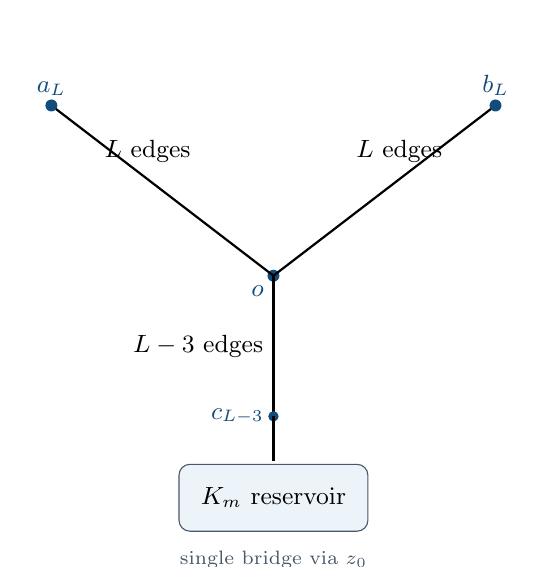
\begin{tikzpicture}[>=Latex,scale=0.94, every node/.style={font=\small}]
 \fill[highlight] (0,0) circle (2.3pt) node[below left] {$o$};
 \draw[thick] (0,0)--(-3,2.3); \draw[thick] (0,0)--(3,2.3);
 \fill[highlight] (-3,2.3) circle (2.3pt) node[above] {$a_L$};
 \fill[highlight] (3,2.3) circle (2.3pt) node[above] {$b_L$};
 \node[sloped,above] at (-1.7,1.4) {$L$ edges};
 \node[sloped,above] at (1.7,1.4) {$L$ edges};
 \draw[thick] (0,0)--(0,-1.9) node[midway,left] {$L-3$ edges};
 \fill[highlight] (0,-1.9) circle (2pt) node[left] {$c_{L-3}$};
 \draw[thick] (0,-1.9)--(0,-2.5);
 \node[draw=slate,rounded corners=4pt,fill=lightblue,minimum width=2.4cm,minimum height=0.85cm] (cl) at (0,-3.0) {$K_m$ reservoir};
 \node[below=0.12cm of cl, text=slate,font=\scriptsize] {single bridge via $z_0$};
\end{tikzpicture}
\caption{The $F_{L,m}$ construction. The lengths denote whole paths; the clique is attached by one bridge and is deliberately placed below the diametral threshold.}
\label{fig:cam}
\end{figure}

\begin{theorem}[Exact clique-reservoir invariants]\label{thm:Fexact}
For every $L\ge4$ and $m\ge3$,
\begin{align}
\diam(F_{L,m})&=2L, & B(F_{L,m})&=\{a_L,b_L\};\label{eq:Fper}\\
b(F_{L,m})&=f(F_{L,m})=3L;\label{eq:Fbf}\\
\avg_{F_{L,m}}(B,V)&=\frac{m(2L-1)+(7L^2-9L+4)/2}{m+3L-3}.\label{eq:Favg}
\end{align}
The common unrounded signed violation of the two original inequalities is
\begin{equation}\label{eq:Fdef}
 D_{L,m}:=2\avg_{F_{L,m}}(B,V)-3L
 =\frac{(L-2)m-2L^2+4}{m+3L-3},
\end{equation}
with the corresponding integer violation exactly $\lceil D_{L,m}\rceil$.
\end{theorem}
\begin{proof}
The tips $a_L,b_L$ are distance $2L$ apart. Every other vertex of the two long arms is at distance at most $2L-1$ from every vertex. Every $c_i$ is at distance at most $L+i\le2L-3$ from the long tips; its distances to the clique are shorter. The bridge endpoint $z_0$ is at distance $2L-2$ from either tip, whereas any other clique vertex is at distance $2L-1$. Distances within the clique are one. Therefore exactly $a_L,b_L$ have eccentricity $2L$, proving \eqref{eq:Fper}.

The path scaffold contains $1+2L+(L-3)=3L-2$ vertices and is a tree. In any induced bipartite graph or induced forest, at most two vertices from $K_m$ may remain, because any three clique vertices induce a triangle. This gives $b,f\le3L$. Keeping all scaffold vertices together with $z_0,z_1$ induces a tree (with pendant edge $z_0z_1$), hence $b=f=3L$.

By symmetry the transmissions from $a_L$ and $b_L$ agree. From $a_L$, the distances to vertices of the two long arms and the center sum to $2L^2+L$; distances to the short arm sum to $\sum_{i=1}^{L-3}(L+i)=(L-3)(3L-2)/2$. The distance to $z_0$ is $2L-2$, while distances to the other $m-1$ clique vertices equal $2L-1$. Thus the transmission is
\[
 \begin{aligned}
 W(a_L)&=2L^2+L+\frac{(L-3)(3L-2)}2+(2L-2)+(m-1)(2L-1)\\
 &=m(2L-1)+\frac{7L^2-9L+4}2.
 \end{aligned}
\]
Dividing by $n-1=m+3L-3$ yields \eqref{eq:Favg}. Subtracting $3L$ from twice this quantity yields \eqref{eq:Fdef}. As $3L$ is integral, $\lceil2\avg(B,V)\rceil-3L=\lceil D_{L,m}\rceil$.
\end{proof}

\subsection{A linear gap and its sharp constant within the family}
\begin{theorem}[Answer to the historical unbounded-gap question]\label{thm:Funbounded}
Put $m=7L$, $G_L:=F_{L,7L}$, and $n_L=10L-2$. Then
\[
\lceil 2\avg_{G_L}(B,V)\rceil-b(G_L)
=\lceil 2\avg_{G_L}(B,V)\rceil-f(G_L)
=\left\lceil\frac{5L^2-14L+4}{10L-3}\right\rceil,
\]
and
\begin{equation}\label{eq:Flinear}
\lim_{L\to\infty}\frac{\lceil2\avg_{G_L}(B,V)\rceil-b(G_L)}{n_L}
=\lim_{L\to\infty}\frac{\lceil2\avg_{G_L}(B,V)\rceil-f(G_L)}{n_L}
=\frac1{20}.
\end{equation}
Consequently the signed violation of each previously false conjecture is unbounded, indeed of linear order.
\end{theorem}
\begin{proof}
Substitute $m=7L$ into \eqref{eq:Fdef} and divide numerator and denominator by $L$. The unrounded violation is $(5L^2-14L+4)/(10L-3)=L/2+O(1)$. Because $n_L=10L-2$, its ratio to $n_L$ tends to $1/20$. Ceiling changes the numerator by less than one. In particular both integer violations diverge.
\end{proof}
\begin{theorem}[Global finite upper bound within the clique family]\label{thm:Fsharp}
For every $L\ge4,m\ge3$ and $n=n(F_{L,m})$,
\begin{equation}\label{eq:Fupper}
D_{L,m}\le\frac{n}{20},\qquad \lceil D_{L,m}\rceil\le\left\lceil\frac n{20}\right\rceil.
\end{equation}
The coefficient $1/20$ is the sharp asymptotic maximum over the entire two-parameter family $\{F_{L,m}\}$.
\end{theorem}
\begin{proof}
Since $m=n-3L+2$, \eqref{eq:Fdef} gives
\[
(n-1)D_{L,m}=-5L^2+(n+8)L-2n
=-5\left(L-\frac{n+8}{10}\right)^2+\frac{(n+8)^2}{20}-2n.
\]
Discard the nonpositive square. Since $n\ge13$, the inequality $64\le23n$ implies
\[
20(n-1)D_{L,m}\le n^2-24n+64\le n^2-n.
\]
Thus $D_{L,m}\le n/20$. The matching limiting fraction is \eqref{eq:Flinear}. This is an optimization \emph{only inside $F_{L,m}$}, not over all connected graphs.
\end{proof}
\begin{remark}[Exact scale optimization]
If $m/L\to\alpha>0$, then $D_{L,m}/n\to(\alpha-2)/(\alpha+3)^2$. Its derivative equals $(7-\alpha)/(\alpha+3)^3$, and the maximum is attained at $\alpha=7$, equal to $1/20$. The finite square-completion proof additionally covers parameters outside this scaling regime.
\end{remark}

\section{Girth-eight reservoirs: exact distance data}
The dense clique is incompatible with girth at least five. A separate construction replaces each edge of a complete bipartite graph by a path of length two. Its high number of subdivision vertices is dominated economically by choosing original endpoints; a pendant path then makes the original distance reference set a singleton without altering the girth.

\begin{definition}[One-subdivision and rooted path]\label{def:J}
Fix $q\ge2$. Let $H_q$ have vertices
\[
X=\{x_1,\ldots,x_q\},\quad Y=\{y_1,\ldots,y_q\},\quad E^*=\{e_{ij}:1\le i,j\le q\},
\]
with exactly the edges $x_i e_{ij}$ and $e_{ij}y_j$. For an integer $L\ge1$, let $J_{q,L}$ be obtained by adding the path
\[
 x_1-p_1-p_2-\cdots-p_L
\]
with $L$ new vertices. We use $\mathcal P=\{p_1,\ldots,p_L\}$ for its vertex set.
\end{definition}
\begin{figure}[H]
\centering
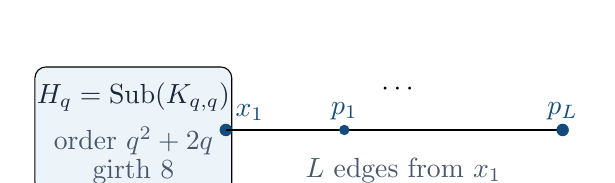
\begin{tikzpicture}[scale=.94]
\node[draw,rounded corners,fill=lightblue,minimum width=2.5cm,minimum height=1.6cm] (H) at (0,0) {};
\node[text=ink] at (0,0.45) {$H_q=\operatorname{Sub}(K_{q,q})$};
\node[text=slate] at (0,-0.15) {order $q^2+2q$};
\node[text=slate] at (0,-0.56) {girth $8$};
\fill[highlight] (1.25,0) circle (2.4pt) node[above right] {$x_1$};
\draw[thick] (1.25,0)--(2.85,0)--(4.35,0)--(5.8,0);
\fill[highlight] (2.85,0) circle (2pt) node[above] {$p_1$};
\node at (3.6,0) [above=9pt] {$\cdots$};
\fill[highlight] (5.8,0) circle (2.4pt) node[above] {$p_L$};
\node[text=slate] at (3.65,-0.55) {$L$ edges from $x_1$};
\end{tikzpicture}
\caption{A subdivided complete bipartite reservoir with one pendant path. The final leaf $p_L$ is the unique minimum-degree vertex.}
\label{fig:J}
\end{figure}

\begin{lemma}[Basic invariants and transmission]\label{lem:base}
For every $q\ge2$ and $L\ge1$,
\begin{align}
N_q&:=|V(H_q)|=q^2+2q,& n_{q,L}&:=|V(J_{q,L})|=N_q+L,\label{eq:Nq}\\
\girth(J_{q,L})&=8,&A(J_{q,L})&=\{p_L\}.\label{eq:Jgirth}
\end{align}
Writing $W_q=\sum_{v\in V(H_q)}\dist_{H_q}(x_1,v)$,
\begin{equation}\label{eq:W}
W_q=3q^2+4q-4.
\end{equation}
The \emph{exact} original set-to-vertex average is
\begin{equation}\label{eq:Javg}
\avg_{J_{q,L}}(A,V)=\frac{N_qL+W_q+L(L-1)/2}{N_q+L-1}.
\end{equation}
\end{lemma}
\begin{proof}
The graph $H_q$ is the one-subdivision of $K_{q,q}$. A shortest cycle of $K_{q,q}$ is a four-cycle, whose length doubles to eight upon subdivision; the appended path creates no new cycle. All original vertices in $H_q$ have degree $q\ge2$ and all subdivision vertices have degree two. The attachment increases the degree of $x_1$ by one, while the internal path vertices have degree two and $p_L$ alone has degree one. This establishes \eqref{eq:Nq}--\eqref{eq:Jgirth}.

From $x_1$, the $q-1$ other $X$-vertices have distance four, the $q$ vertices in $Y$ have distance two, the $q$ vertices $e_{1j}$ have distance one, and the other $q(q-1)$ subdivision vertices have distance three. Thus
\[
W_q=4(q-1)+2q+q+3q(q-1)=3q^2+4q-4.
\]
From $p_L$, the distances to the $N_q$ vertices of $H_q$ sum to $N_qL+W_q$, and those to $p_1,\ldots,p_{L-1}$ sum to $L(L-1)/2$. Division by $n_{q,L}-1$ gives \eqref{eq:Javg}.
\end{proof}

\section{Exact total domination: a parity-and-cover principle}
The earlier version of this manuscript used only an explicit upper bound on $\gam(J_{q,L})$. The next two proofs close that missing exactness issue for \emph{every} $q\ge2$ and $L$ divisible by four. No numerical optimization is needed.

\begin{lemma}[Four-block path parity]\label{lem:path}
Let $L=4s$ with $s\ge1$, and let $D$ be a total dominating set of $J_{q,L}$. Write $P_D=D\cap\mathcal P$.
\begin{enumerate}[label=(\roman*)]
\item Always $|P_D|\ge2s=L/2$, regardless of whether $x_1\in D$.
\item If $x_1\notin D$ and $p_1\in D$, then $|P_D|\ge2s+1=L/2+1$.
\end{enumerate}
\end{lemma}
\begin{proof}
There are exactly $2s$ even-index path vertices $p_2,p_4,\ldots,p_{4s}$ and $2s$ odd-index vertices $p_1,p_3,\ldots,p_{4s-1}$. The only neighbors of any even-index path vertex are odd-index path vertices. Each selected odd-index vertex can dominate at most two even-index vertices. Hence at least $s$ odd-index path vertices belong to $D$.

Every odd-index path vertex other than $p_1$ must be dominated by a selected even-index path vertex. Even if $p_1$ is dominated by the outside root $x_1$, there remain $2s-1$ odd-index path vertices to dominate; each selected even-index vertex can dominate at most two. Therefore at least $\lceil(2s-1)/2\rceil=s$ even-index path vertices belong to $D$, proving (i).

If $p_1\in D$, the selected odd-index vertex $p_1$ can dominate \emph{only one} even-index path vertex, namely $p_2$. Were exactly $s$ odd-index path vertices selected, they could dominate at most $1+2(s-1)=2s-1$ even-index vertices, a contradiction. Thus at least $s+1$ odd-index path vertices are selected. Since $x_1\notin D$, all $2s$ odd-index path vertices (including $p_1$) must be dominated by selected even-index path vertices, of which there are at least $s$. The total is at least $2s+1$, proving (ii).
\end{proof}

\begin{theorem}[\textbf{Exact total-domination number}]\label{thm:gamma}
For all integers $q\ge2$ and $s\ge1$,
\begin{equation}\label{eq:gammaexact}
\boxed{\gam(J_{q,4s})=2q+2s=2q+\frac L2.}
\end{equation}
\end{theorem}
\begin{proof}
\emph{Upper bound.} Take all $q$ vertices of $X$, the $q$ diagonal subdivision vertices $e_{ii}$, and, for each $j=0,\ldots,s-1$, the path pair $p_{4j+2},p_{4j+3}$. Every $e_{ij}$ has selected neighbor $x_i$, every $x_i$ has selected neighbor $e_{ii}$, and every $y_j$ has selected neighbor $e_{jj}$. The pairs cover the consecutive path blocks $p_{4j+1},\ldots,p_{4j+4}$, including the selected vertices themselves. This is a total dominating set of size $2q+2s$.

\emph{Lower bound.} Let $D$ be any total dominating set, and split it into the core part $D_H=D\cap V(H_q)$ and path part $P_D=D\cap\mathcal P$. To dominate every subdivision vertex $e_{ij}$, at least one of its only two neighbors $x_i,y_j$ must lie in $D$. Therefore either $X\subseteq D$ or $Y\subseteq D$: otherwise a missing $x_i$ and a missing $y_j$ would leave $e_{ij}$ undominated.

If $X\subseteq D$, all $q$ vertices $y_j$ must each be dominated by a subdivision vertex in $D$; a single $e_{ij}$ is adjacent to only one $y_j$. Hence $|D_H|\ge2q$. By \cref{lem:path}(i), $|P_D|\ge2s$ and thus $|D|\ge2q+2s$.

If $Y\subseteq D$, each of $x_2,\ldots,x_q$ must be dominated by a subdivision vertex of $D$, so $|D_H|\ge q+(q-1)=2q-1$. If $|D_H|\ge2q$, again apply \cref{lem:path}(i). The sole remaining case is $|D_H|=2q-1$. Then $D_H$ consists of all $q$ vertices of $Y$ and exactly one subdivision vertex incident to each of $x_2,\ldots,x_q$, with no original $X$-vertex and no $e_{1j}$. In particular, $x_1$ has no selected core neighbor. As $x_1$ must be dominated, $p_1\in D$, while $x_1\notin D$. By \cref{lem:path}(ii), $|P_D|\ge2s+1$, giving $|D|\ge(2q-1)+(2s+1)=2q+2s$. This exhausts all possibilities and matches the explicit upper bound.
\end{proof}
\begin{remark}[Why a single saved core vertex does not help]
The apparent option of choosing all of $Y$ and only $q-1$ subdivision vertices saves one vertex in the core. The necessary choice $p_1\in D$ then incurs exactly one additional path cost by the parity lemma. The matching loss-and-compensation estimate is the substantive point that turns an upper bound into the exact formula.
\end{remark}

\section{Exact violations and the sharp $1/8$ coefficient}
\begin{definition}[Signed and integer deficits]\label{def:deficit}
For $q\ge2$ and $L\equiv0\pmod4$ put $n=N_q+L$, and define the unrounded and integer deficits of the unchanged original \#267 inequality by
\[
\Def_{q,L}:=\avg_{J_{q,L}}(A,V)-\gam(J_{q,L}),\qquad
\widehat\Def_{q,L}:=\left\lceil\avg_{J_{q,L}}(A,V)\right\rceil-\gam(J_{q,L}).
\]
Since $\gam(J_{q,L})$ is an integer, $\widehat\Def_{q,L}=\lceil\Def_{q,L}\rceil$.
\end{definition}

\begin{theorem}[Exact deficit formula]\label{thm:defexact}
For every $q\ge2$ and $4\mid L$, writing $n=q^2+2q+L$, the two deficits are
\begin{equation}\label{eq:Delta}
\boxed{\Def_{q,L}=\frac{(q^2+2q)L}{2(n-1)}+\frac{3q^2+4q-4}{n-1}-2q,\qquad
\widehat\Def_{q,L}=\lceil\Def_{q,L}\rceil.}
\end{equation}
\end{theorem}
\begin{proof}
Insert \eqref{eq:Javg} and \eqref{eq:gammaexact}. In the difference $\avg(A,V)-L/2$, the path's quadratic distance sum cancels exactly:
\[
N_qL+W_q+\frac{L(L-1)}2-\frac L2(N_q+L-1)=\frac{N_qL}2+W_q.
\]
Subtract $2q$ and divide by $n-1$. No approximation occurs.
\end{proof}
\begin{theorem}[Sharp finite-size bound within the entire family]\label{thm:sharp8}
For every $q\ge2$, every positive $L$ divisible by four, and $n=|V(J_{q,L})|$,
\begin{equation}\label{eq:bound8}
\Def_{q,L}\le\frac n8,\qquad \widehat\Def_{q,L}\le\left\lceil\frac n8\right\rceil.
\end{equation}
Moreover $1/8$ is the exact largest asymptotically achievable normalized deficit \emph{within the whole family $\{J_{q,L}:q\ge2,\ 4\mid L\}$}.
\end{theorem}
\begin{proof}
Write $N=N_q$ and $W=W_q$. By arithmetic-geometric mean, $NL\le(N+L)^2/4=n^2/4$. The explicit transmission satisfies $W=3q^2+4q-4\le3(q^2+2q)=3N\le3n$, and $2q\ge4$. Consequently \eqref{eq:Delta} gives
\[
\Def_{q,L}\le\frac{n^2}{8(n-1)}+\frac{3n}{n-1}-4
=\frac{n^2-8n+32}{8(n-1)}\le\frac{n}{8},
\]
where the last inequality holds whenever $7n\ge32$ and our graphs have $n\ge12$. Monotonicity of ceiling gives the integer upper bound. The matching asymptotic construction is provided in \cref{thm:attain8}, which shows sharpness. No universal claim is made over graphs outside this two-parameter family.
\end{proof}

\begin{theorem}[Explicit linear counterexamples, optimal family coefficient]\label{thm:attain8}
For every integer $t\ge4$, choose
\[
q=2t,\qquad L=4t^2,\qquad Q_t:=J_{2t,4t^2},\qquad n_t=8t^2+4t.
\]
Then $Q_t$ has girth eight and a unique minimum-degree vertex, and
\begin{align}
\gam(Q_t)&=2t^2+4t,\label{eq:Qtgam}\\
\avg_{Q_t}(A,V)&=\frac{24t^4+16t^3+10t^2+8t-4}{8t^2+4t-1},\label{eq:Qtavg}\\
\widehat\Def(Q_t)&=\left\lceil\frac{4(2t^4-6t^3-t^2+3t-1)}{8t^2+4t-1}\right\rceil>0.\label{eq:Qtdef}
\end{align}
In particular, each $Q_t$ is a counterexample to the \emph{original} WOWII \#267 statement, and
\begin{equation}\label{eq:Qtlimit}
\lim_{t\to\infty}\frac{\widehat\Def(Q_t)}{n_t}=\frac18.
\end{equation}
The exact signed deficit also satisfies, for every $t\ge4$,
\begin{equation}\label{eq:quantfinite}
\Def(Q_t)>\frac{n_t}{8}-4t.
\end{equation}
\end{theorem}
\begin{proof}
From \cref{lem:base} one has $N=4t^2+4t$, $W=12t^2+8t-4$, $L=4t^2$, and $n=N+L=8t^2+4t$. The exact value \eqref{eq:Qtgam} follows from \cref{thm:gamma}. Substitution into \eqref{eq:Javg} yields \eqref{eq:Qtavg}, and subtracting \eqref{eq:Qtgam} yields \eqref{eq:Qtdef}.

The numerator $2t^4-6t^3-t^2+3t-1=2t^3(t-3)-t^2+3t-1$ is positive for $t\ge4$, so the strict counterexample statement follows. Polynomial division produces the useful exact identity
\[
\Def(Q_t)=t^2-\frac{7t}{2}+\frac{11}{8}+\frac{3t-21/8}{8t^2+4t-1}.
\]
The last two terms have positive sum for $t\ge4$, while $n_t/8-4t=t^2-7t/2$; hence \eqref{eq:quantfinite}. Dividing the exact polynomial expressions by $n_t$ gives $\Def(Q_t)/n_t\to1/8$. The ceiling changes this ratio by less than $1/n_t$, proving \eqref{eq:Qtlimit}.
\end{proof}

\begin{corollary}[Correction and completion of the former $2/25$ claim]\label{cor:old}
Consider the earlier specialization $q=4t$, $L=4t^2$, denoted $J_t$ in the previous edition. Its earlier \emph{upper bound} is in fact exact:
\[
\gam(J_t)=2t^2+8t\quad (t\ge1),\qquad
\lim_{t\to\infty}\frac{\lceil\avg_{J_t}(A,V)\rceil-\gam(J_t)}{|V(J_t)|}=\frac{2}{25}.
\]
The new choice $q=2t$ achieves the strictly larger limiting ratio $1/8$.
\end{corollary}
\begin{proof}
Apply \cref{thm:gamma} with $q=4t$, $L=4t^2$. In this case $N=16t^2+8t$, $n=20t^2+8t$, and the leading contribution to \eqref{eq:Delta} is $NL/[2(n-1)]\sim(8/5)t^2$, while $W/(n-1)=O(1)$ and $2q=8t$. After division by $n\sim20t^2$ the ratio tends to $(8/5)/20=2/25$. Finally $2/25<1/8$.
\end{proof}

\section{Independent computational spot checks}
The mathematical arguments in \cref{thm:Fexact,thm:Fsharp,thm:gamma,thm:sharp8,thm:attain8} are symbolic and uniform; a finite search is not used to close any quantifier. Exact-rational arithmetic independently checks the displayed specializations. Some results follow.
\begin{center}
\small
\begin{tabular}{rrrrrr}
\toprule
$L$ & $m$ & $n(F_{L,m})$ & $b=f$ & $\avg(B,V)$ & signed integer violation \\
\midrule
4 & 3 & 13 & 12 & $61/12$ & $-1$\\
4 & 28 & 38 & 12 & $236/37$ & $1$\\
5 & 35 & 48 & 15 & $382/47$ & $2$\\
10 & 70 & 98 & 30 & $1637/97$ & $4$\\
20 & 140 & 198 & 60 & $6772/197$ & $9$\\
\bottomrule
\end{tabular}
\end{center}
\begin{center}
\small
\begin{tabular}{rrrrrr}
\toprule
$t$ & $q$ & $L$ & $n(Q_t)$ & $\gam(Q_t)$ & exact integer violation \\
\midrule
3 & 6 & 36 & 84 & 30 & $0$\\
4 & 8 & 64 & 144 & 48 & $4$\\
5 & 10 & 100 & 220 & 70 & $9$\\
10 & 20 & 400 & 840 & 240 & $67$\\
16 & 32 & 1024 & 2112 & 576 & $202$\\
24 & 48 & 2304 & 4704 & 1248 & $494$\\
40 & 80 & 6400 & 12960 & 3360 & $1462$\\
\bottomrule
\end{tabular}
\end{center}
The $t=3$ row is a boundary sanity check: the limiting family need not refute the conjecture at every smaller parameter. It is the \emph{proved} $t\ge4$ range that establishes the counterexample theorem. Independently, a binary mixed-integer optimization of the vertex-by-open-neighborhood incidence matrix recovered $\gam(J_{q,L})=2q+L/2$ for every tested $q\in\{2,3,4,5\}$, $L\in\{4,8,12,16\}$; this numerical test is supportive only.

The following Python 3 standard-library snippet reproduces the exact rational deficits in the two tables. It is embedded here so the manuscript remains a \emph{single} compilable \texttt{.tex} file; it requires no separate data, bibliography, or code file.
\begin{lstlisting}[style=pcode,language=Python]
from fractions import Fraction
from math import ceil

def peripheral(L, m):
    n = m + 3*L - 2
    avg = Fraction(2*m*(2*L-1) + 7*L*L - 9*L + 4,
                   2*(n-1))
    return n, 3*L, avg, ceil(2*avg)-3*L

def domination(q, L):
    assert q >= 2 and L > 0 and L % 4 == 0
    N, W = q*q + 2*q, 3*q*q + 4*q - 4
    n = N + L
    avg = Fraction(N*L + W + L*(L-1)//2, n-1)
    gamma = 2*q + L//2
    return n, gamma, avg, ceil(avg)-gamma

for L, m in [(4,3),(4,28),(5,35),(10,70),(20,140)]:
    print("F", L, m, peripheral(L, m))
for t in [3,4,5,10,16,24,40]:
    print("Q", t, domination(2*t, 4*t*t))
\end{lstlisting}

\section{Method transfer, novelty, and G1--G6 research audit}
The mathematical mechanism has two complementary parts. For \#21 and \#42, \emph{peripheral shielding} fixes the true extremal distance reference set while a clique contributes many distant vertices but at most two to either maximal induced bipartite order or maximal induced forest. Exact arithmetic and two-parameter optimization replace a single isolated counterexample by a linear sequence. For \#267, \emph{girth repair} replaces the clique by the subdivision of $K_{q,q}$, and \emph{cover--parity locking} proves the exact total-domination number. The decisive new proof ingredient in this edition is the collision between the core vertex-cover requirement and the exceptional path cost when $p_1$ must be selected.

The supplied \emph{Verifiable Mathematical Reasoning Corpus} includes the research notes [015] \emph{One Missing Edge}, [034] \emph{Global Proof Transfers}, and [040] \emph{OEIS Conjecture Hunt}, which informed the strategy of transferring exact defect calculations between settings \cite{corpus}. We do \emph{not} assume any unverified statement from those research drafts as a lemma. Every graph-theoretic identity needed here is proved inside this manuscript. The repository's own provenance text describes its contents as research drafts rather than peer-reviewed results \cite{corpus}.

\begin{table}[H]
\centering\small
\begin{tabularx}{\textwidth}{@{}p{0.09\textwidth}p{0.26\textwidth}X@{}}
\toprule
Gate & Assessment & Specific evidence and limitation\\
\midrule
G1 & \textbf{Partial} & The three original problems are historical numbered named conjectures. The unbounded-gap follow-up to \#21/\#42 was explicitly asked historically but does not have its own independently numbered conjecture entry.\\
G2 & \textbf{Met} & Original $b$, $f$, $\gam$, girth, periphery, minimum-degree set, distance averages and ceilings are used unchanged.\\
G3 & \textbf{Not met for first resolution} & \#21/\#42 were refuted in 2008. \#267 has public August 2026 counterexamples even though the maintained list's status remains ``open''.\\
G4 & \textbf{Met for our quantified claims} & Exact invariants, exact $\gam$, sharp family-specific coefficients, and all-parameter counterexamples have full unconditional proofs. This does not constitute a first solution to a still-open original named conjecture.\\
G5 & \textbf{Concrete strengthening; novelty unverified} & The exact $\gam=2q+L/2$, parity compensation, $n/8$ within-family upper bound, and matching asymptotic lower bound are more than coordinate changes. A systematic priority comparison is still required.\\
G6 & \textbf{Not certified} & Public targeted searches do not rule out earlier unpublished or unindexed quantitative constructions. Neither first-priority authorship nor independently verified originality is asserted.\\
\bottomrule
\end{tabularx}
\caption{Strict evaluation against the user's six conditions. The original named-conjecture standard is not weakened by the creation of auxiliary problems.}
\label{tab:gates}
\end{table}

\paragraph{What is and is not settled.} The published 2008 question whether the violations of \#21 and \#42 can grow without bound receives an explicit affirmative answer in \cref{thm:Funbounded}. The unchanged \#267 statement has infinitely many exact, girth-eight counterexamples in \cref{thm:attain8}; its previous public refutation precludes a first-solution claim. We do \emph{not} claim a new true theorem replacing a false conjecture, a universal $n/8$ maximum over all graphs, an exact global extremal characterization, a machine-checked Lean proof, formal peer review, or priority independently established against the complete literature.

\section{Conclusions and remaining frontier}
The first construction yields an unconditional, simultaneous, linear-order violation of two 2003--2004 conjectures and a matching upper-bound coefficient of $1/20$ within its entire class. The second supplies a girth-eight class with \emph{exact} total domination and an exact signed violation formula for a 2007 conjecture, whose normalized coefficient is sharply $1/8$ inside the two-parameter class. This is a strict mathematical extension of the previous $2/25$ one-sided estimate: the domination number is now known exactly and the reservoir geometry is optimized.

The genuine open mathematical next step is \emph{not} to relabel these already false originals as open. It is to transfer cover--parity locking or peripheral shielding into a distinct historical conjecture whose pre-resolution open status can be independently verified, then obtain an original unconditional full proof. In the present manuscript the all-six-gates (G1--G6) first-solution criterion remains unmet, even though its new auxiliary theorems are fully proved.

\begin{thebibliography}{9}
\bibitem{wowii} E.~DeLaVi\~na, \emph{Written on the Wall II: Conjectures of Graffiti.pc}, University of Houston--Downtown, maintained list, snapshot printed 6 November 2026; original conjecture entries 21, 42, and 267 (and comments under 21 and 42). \url{https://www.uhd.edu/academics/sciences/mathematics-statistics/wowii/files/wowiiaii.pdf}.
\bibitem{village} \emph{Grok AI Village News}, ``Graffiti.pc 267 FALSE,'' dispatch 4240, 24 August 2026, publicly reporting earlier explicit counterexamples and computational checks. \url{https://grok-ai-village-news-496089.gitlab.io/series/wow.html}. Not treated as a peer-reviewed proof of the present results.
\bibitem{mathbench} \emph{MathBench}, ``Size and Number of Smallest Counterexamples to a Total Domination Average Distance Conjecture,'' MB13-OWN-P021, publicly identifying WOWII 267 as false. \url{https://mathbench.ai/en/items/MB13-OWN-P021}. A problem benchmark, not a peer-reviewed first-priority certificate.
\bibitem{corpus} QEEDDD, \emph{Verifiable Mathematical Reasoning Corpus}, GitHub, including manuscripts [015], [034], [040], accessed 17 November 2026. The repository describes the works as unrefereed research drafts. \url{https://github.com/QEEDDD/Verifiable-Mathematical-Reasoning-Corpus}.
\end{thebibliography}
\end{document}
